\documentclass[useAMS,usenatbib]{mn2e}
\usepackage{myaasmacros}
\usepackage{graphicx}
\usepackage{ulem}
\usepackage{amsmath}
\usepackage{multirow}

% Some definitions of things I always use here:
\def\ltsima{$\; \buildrel < \over \sim \;$}
\def\simlt{\lower.5ex\hbox{\ltsima}}   
\def\gtsima{$\; \buildrel > \over \sim \;$}
\def\simgt{\lower.5ex\hbox{\gtsima}}

%Code definition:
\def\Glass{{\sc Glass}}
\def\PixeLens{{\sc PixeLens}}

\title[Light versus Dark in Strong Lensing Galaxies]{Light versus Dark in Strong Lensing Galaxies: Dark matter halos that are rounder than their stars}

\author[Bruderer]{Claudio Bruderer$^{1}$\thanks{E-mail: claudio.bruderer@phys.ethz.ch}, J. I. Read$^{1,2}$, P. Saha$^{3}$, J. Coles$^{4}$\\
$^{1}$Institute for Astronomy, Department of Physics, ETH Z\"urich, Wolfgang-Pauli-Strasse 27, CH-8093 Z\"urich, Switzerland\\
$^{2}$Department of Physics, University of Surrey, Guildford, GU2 7XH, UK\\
$^{3}$Institute for Theoretical Physics, University of Z\"urich, Winterthurerstrasse 190, 8057 Z\"urich, Switzerland\\
$^{4}$Exascale Research Computing Lab, Campus Teratec, 2 Rue de la Piquetterie, 91680 Bruyeres-le-Chatel, France
}

\begin{document}

\maketitle

\begin{abstract}
We measure the shape and alignment of stars and dark matter in 11 strong
lensing galaxies, finding in all cases that the dark matter halos are rounder
than the light distribution over the range $R_e < R < 5R_e$.  Averaging over
larger radii, the lenses become increasingly elliptical both in their dark
matter and stellar components, as defined using the ratio $s$ of the largest to
smallest eigenvalues of the 2D moment of inertia tensor of the projected
lensing mass.  While dark matter halos are never more elliptical than $s_{dm} =
1.15$, their stars can extend to $s_* > 1.4$ Three systems, in particular, have
very high stellar ellipticity ($s_* > 1.6$) and correspondingly high alignment
between light and dark. One of these -- B1608 -- is a known merging pair; we
suggest that the other two (B0712 and B2016) may also be recent post-merger
systems.  Galaxies with high dark matter ellipticity and weak external shear
show very strong alignment between light and dark; those with strong shear
($\gamma \simgt 0.1$) can be very highly misaligned. This is reassuring since
isolated misaligned galaxies are expected to be unstable. 

Our results provide a new constraint on galaxy formation models that must
explain the origin of both very round dark matter halos and highly misaligned
strong lensing systems. Such misalignments also present a new challenge for alternative
gravity theories in which the light and dark must necessarily be highly
correlated.

\end{abstract}

\begin{keywords}
Gravitational lensing: strong --- galaxies: structure
\end{keywords}


\section{Introduction}\label{sec:introduction}

The ellipticity and shape of stars relative to their host dark matter halo encodes information both about our cosmological model ($\Lambda$CDM) and galaxy formation \citep[e.g.][]{1994ApJ...431..617D,2001ApJ...551..294I,2004ApJ...611L..73K,2007MNRAS.378...55M,2007arXiv0707.0737D,2012MNRAS.424L..16L,2014JPhG...41f3101R}. `Dark-matter-only' (DMO) simulations in $\Lambda$CDM predict dark matter halos that are triaxial \citep{1991ApJ...378..496D,1992ApJ...399..405W,1996ApJ...462..563N,2002ApJ...574..538J}, with mean `shape parameter' $\langle q \rangle = (b+c)/2a \sim 0.8$ (where $a > b > c$ are the long, intermediate and short axes of the figure; \citealt{2007MNRAS.378...55M}). This corresponds to a typically {\it prolate} halo. However, including `baryons' (stars and gas) in the models produces halos that are significantly rounder and -- at least for disc galaxies -- well-aligned with the light distribution \citep{1991ApJ...377..365K,1994ApJ...431..617D,2007arXiv0707.0737D}. Halo shapes and alignments also constrain alternative gravity models \citep{2001MNRAS.327..552M,2004ApJ...610L..97H,2005MNRAS.361..971R,2012PhRvD..86h3507F,2013MNRAS.434.2971D}. If the visible light is the only source of gravity in a galaxy, then we expect the light and mass distribution to be highly correlated; if dark matter is present, however, such correlations can at least in principle be broken.

Strong lensing provides a unique probe of the alignment and shape of the total mass distribution in galaxies \citep[e.g.][]{1986ApJ...310..568B,1992grle.book.....S,1998ApJ...509..561K,2000ApJ...543..131K,2006ApJ...649..599K,2007AJ....134..668A,2008MNRAS.383..857F,2010ApJ...724..511A,2012MNRAS.424..104L}. For `red and dead' ellipticals that are largely devoid of gas, their baryonic content can be mapped through stellar population synthesis modelling of their light distribution alone \citep[e.g.][]{2005ApJ...623L...5F,2006ApJ...640..662T,2008MNRAS.383..857F}. Furthermore, such systems are dense enough to produce strong lensing, opening up the possibility of directly comparing the light and mass in these galaxies \citep{1998ApJ...509..561K,2008MNRAS.383..857F,2009ApJ...690..670T,2012A&A...538A..99S}. Previous work in the literature has found that the light and mass are well-aligned (though a mis-match of up to 10$^\circ$ is not uncommon; e.g. \citealt{2012A&A...538A..99S}). However, results on the ellipticity of light and mass agree less well, with \citet{2012A&A...538A..99S} finding a strong correlation and \citet{1998ApJ...509..561K} and \citet{2008MNRAS.383..857F} finding none. It is difficult, however, to compare the results between these different studies because they use different lens modelling techniques; different definitions of ellipticity; and different radii over which the shapes and alignments are probed. Furthermore, none to date have applied their methodology to mock data to determine the robustness of the results.

Weak lensing can also be used to probe the shape and alignment between light and dark, but only for `stacked' galaxies \citep{2000astro.ph..6281B,2000ApJ...538L.113N}. \citet{2004ApJ...606...67H} applied this idea to data from the Red-Sequence Cluster Survey (RCS) to measure the first weak lensing signal of halo flattening. They found that dark matter halos appear to be rounder then their light distributions, with some weak evidence for alignment. Both measurements are challenging, however, and more recent data appear to be at odds with this early work, favouring dark matter halos that are more elliptical than their stars \citep{2006MNRAS.370.1008M,2007ApJ...669...21P,2012A&A...545A..71V}.

Recently, we introduced a new non-parametric lens tool, \Glass\ \citep{2014arXiv1401.7990C}. Applying this to a large suite of mock data, we showed that mass and light can only reliably be disentangled in strong lensing systems if: i) there are at least four images; and ii) time delay data are available and/or the stellar mass contributes significantly to the potential. In this paper, we collate data of the above quality, compiling a sample of 11 strong lens galaxies. We apply \Glass\ to these lenses to non-parametrically measure the shape and alignment of the stars and {\it dark matter}  in these lensing galaxies, for the first time. This differs from previous works that have all compared the light distribution with the total mass, rather than the dark matter. Since the stars often dominate the central potential, the total mass naturally correlates with the light, potentially masking theoretically interesting results about the dark matter distribution. Our comparison between light and dark is made possible by the fact that \Glass\ uses the light distribution as a prior on the mass map, ensuring that the dark matter mass is always positive.

This paper is organised as follows. In \S\ref{sec:glass}, we briefly review the \Glass\ code. In \S\ref{sec:data}, we present our data compilation with references. In \S\ref{sec:results}, we present our results. Finally, in \S\ref{sec:conclusions} we discuss the implications of these results and we present our main conclusions.

\section{\Glass: A non-parametric lens tool}\label{sec:glass}

\Glass{} is a new `non-parametric' gravitational lens modelling framework
\citep{2014arXiv1401.7990C} generates a distribution of
mass models given a set of basic assumptions, or priors. Hence, \Glass\ does not yield the most probable mass model. Rather, it calculates an ensemble of all allowed models given the data and assumed priors. In this context,
`non-parametric' really just mean that many more parameters than data constraints are used
such that system of equations describing the lensing mass distribution is
under-constrained. \Glass{} shares some aspects with an earlier code
\PixeLens{} \citep{2004AJ....127.2604S,2008ApJ...679...17C}, but has a completely
different code base. Its key improvements upon \PixeLens{} which are relevant
for this paper include:

\begin{enumerate}
\item A new uniform sampling algorithm for high
    dimensional spaces \citep{2012MNRAS.425.3077L}. This allows for large
    ensembles of $>10,000$ models to be efficiently generated. 
%\item \Glass\ provides a modular framework that allows new priors to be added
%    and modified easily.
%\item The basis functions approximating a model can be easily changed (in this
%    paper, we assume pixels as in \PixeLens). 
\item With so many models in the final ensemble, we can afford to apply
    non-linear constraints (for example stellar kinematic data; or the removal of
    models with spurious extra images) to accept/reject models in a post-processing
    step.
\item The central region of the mass map can have a higher resolution to more
    efficiently capture steep models.
\item Stellar density can be used as an additional lower-bound constraint on the models. 
%\item Point or extended mass objects can be placed in the field.
\end{enumerate} 

%\Glass{} is described in detail in the code paper: \citet{2014arXiv1401.7990C}.
In this paper, the default priors used to model each lens are listed below.  Table
\ref{tab:lenspriors} identifies lenses for which we have modified these defaults.
For each lens we assume:

\begin{enumerate} 
\item Observational priors (redshifts, image positions relative to lens position).
\item Image parity is enforced.
\item A reconstructed stellar mass map as lower mass bounds in every pixel.
\item The local density gradient is always pointing within 50$^{\circ}$ to the center and the slope is at most 0 everywhere. In other words, the density profile peaks in the center.
\item The fixed cosmology $\Omega_{m} = 0.28$, $\Omega_{\Lambda} = 0.72$, $\Omega_{k} = 0$, $H_{0}^{-1} = 13.7$ Gyr.
\item A flat prior on the magnitude of the external shear $|\gamma|$ on $[0,1]$.
\end{enumerate}

In cases where more information is available, the following priors are also used:

\begin{enumerate}
\item[(vii)] A flat prior on measured time delays within the $\pm 1\sigma$-interval.

% \item[(viii)] External point masses to model satellite galaxies outside but
% close to the Einstein radius.

\item[(viii)] Point symmetry $\kappa(x,y) = \kappa(-x,-y)$ where 
the surface mass profile can be assumed to be symmetric (3+1 quad
configurations and the double \textit{Q0957}).

\end{enumerate}

\subsection{Measuring the shape and alignment of a lens}\label{sec:shapemethod}
We employ the same shape definition as in \citep{2014arXiv1401.7990C}. The shape parameter $s$ is defined as the ratio of the two eigenvalues $\lambda_1$ and $\lambda_2$, i.e.
\begin{equation}\label{eq:shapeestimate}
    s \equiv \frac{\lambda_{1}}{\lambda_{2}}, \ \ \ \mathrm{where} \ \lambda_{1} \geq \lambda_{2},
\end{equation}
of the inertia tensor of a mass distribution $M(\boldsymbol{\theta})$
\begin{equation}\label{eq:inertiatensor}
    I = \begin{pmatrix} \sum_\theta M(\boldsymbol{\theta})\theta^{2}_{y} & -\sum_\theta M(\boldsymbol{\theta})\theta_{x}\theta_{y} \\
                        -\sum_\theta M(\boldsymbol{\theta})\theta_{x}\theta_{y} & \sum_\theta M(\boldsymbol{\theta})\theta^{2}_{x} \end{pmatrix}.
\end{equation}
We use these estimators to quantify the shape of the stellar mass distribution and the dark matter distribution. We estimate the latter by reconstructing the total mass distribution with a lower mass prior from the stellar mass distribution and then subtracting the latter off. The shapes of the distributions are computed for all the pixels up to the outermost lensed image and for the pixels within different multiples of the half-light radius $R_e$. $R_e$ is the Petrosian radius containing half of the flux of the total light distribution. As terms in Eq.~\ref{eq:inertiatensor} are weighted with $r^2$, the outer pixels tend to dominate the estimate of the averaged shape within the considered radius. The shape estimates do not necessarily need to be the same within different radii -- e.g. effects such as isophotal twist \citep[e.g.][and references therein]{1978ComAp...8...27B} can cause differences in the shape estimates between the central and the outer parts of the system.

Throughout this paper, we consider only the masses in the pixels up to one pixel length past the outermost image. We generate in each case an ensemble of 10,000 mass models.

\section{Data}\label{sec:data}
Stellar mass maps are taken from \citep{2011ApJ...740...97L}. In that work, the light of the galaxy images in all available HST bands was first fitted using using GALFIT \citep{2002AJ....124..266P}, and the resulting light maps were used to obtain stellar mass maps using a synthesis of the stellar-population models of \citep{2003MNRAS.344.1000B}. The population synthesis marginalised over the star formation epoch and time scales and over the stellar metallicity. The IMF was taken to be the log-normal form given by \citep{2003PASP..115..763C}; a more bottom-heavy IMF would change the mass normalisation \citep[cf.][]{2014ApJ...793...96S} but not the inferred shape of the stellar mass.

As shown in \citep{2014arXiv1401.7990C}, the recovery of the shape information of the lens is only good if there are at least four images. Therefore, we only consider the quad lenses and the twin double \textit{Q0957+561} out of the sample presented in \citep{2011ApJ...740...97L}. This leads to a sample of 11 lenses. We discuss each of these systems, next.

\textit{Q0047-2808} (hereafter \textit{0047}) is a luminous early-type galaxy \citep{1996MNRAS.278..139W}. It is part a group of 9 members, all of which are spectroscopically confirmed \citep{2011ApJ...726...84W}.

\textit{MG0414+0534} (hereafter \textit{0414}) is a passively evolving early-type galaxy \citep{1999AJ....117.2034T}. A very close luminous satellite galaxy was found north-west of the lens \citep{1993AJ....105....1S}. It, however, is more likely a foreground object \citep{2011MNRAS.413L..86C}.

\textit{B0712+472} (hereafter \textit{0712}) is an early-type galaxy \citep{1998AJ....115..377F}.

\textit{RXJ0911+0551} (hereafter \textit{0911}) is an almost circular early-type galaxy \citep{2012A&A...538A..99S}. It has measured time delays \citep{2002ApJ...572L..11H}. It lies on the outskirts of a cluster \citep{2001ApJ...555....1M}. X-ray emission can be detected and an analysis of which yields a temperature of 2.3 keV. There is also a satellite galaxy to the northwest \citep{2000ApJ...544L..35K}.

\textit{Q0957+561} (hereafter \textit{0957}) is a cD galaxy lying close to the centre of a cluster with a high spiral galaxy-fraction \citep[e.g.][]{1992MNRAS.254P..27G,1994A&A...291..411A,1998ApJ...504..661C}. Due to the large image separation, large physical scales are probed. As listed in Table 3 of \cite{2000ApJ...542...74K}, the position angles to the centre of the cluster of earlier lens reconstructions range between 51.8 deg and 67.8 deg measured north-through-east. These results are consistent with the centre of the X-ray emission from the cluster \citep{1998ApJ...504..661C}. The lens has a measured time delay \citep[e.g.][]{2012A&A...540A.132S}. They however also find a three-day lag between the g- and r-bands, a disagreement at the 2$\sigma$-level. They argue that this effect can be accounted for by the presence of a substructure and chromatic dispersion. We find that the results do not change significantly for either estimate and choose therefore the g-band measurement.

\textit{PG1115+080} (hereafter \textit{1115}) is an early-type galaxy \citep{2005ApJ...626...51Y}. It has measured time delays. In this work use recent estimates of the time delays by \cite{2010MNRAS.406.2764T} that differ from previously found values by e.g. \cite{1997ApJ...489...21B}. The environment of the lens was analysed thoroughly \citep{2006ApJ...641..169M,2011ApJ...726...84W}. It is part of a small group of 13 members. Also, X-ray emission was detected from the corresponding group and it yields a temperature of 0.8 keV \citep{2004ApJ...610..686G}.

\textit{B1422+231} (hereafter \textit{1422}) is an early-type galaxy \citep{1996ApJ...462L..53I}. Although there are measured time delays \citep{2001MNRAS.326.1403P}, they seem to deviate significantly from theoretical expectations \citep{2003AJ....126...29R}. We choose therefore not to include them in the analysis. The lens is part of a group with 16 spectroscopically confirmed member galaxies \citep{2006ApJ...641..169M}. Using newer data, an additional member could be found \citep{2011ApJ...726...84W}. \cite{2004ApJ...610..686G} also detect X-ray emission from the corresponding group at a temperature of 1.0 keV.

\textit{B1608+656} (hereafter \textit{1608}) consists of two merging galaxies. The main galaxy is an early-type galaxy which is disrupted by a smaller, probably late-type galaxy \citep{2003ApJ...584..100S}. The system has measured time delays \citep{2002ApJ...581..823F}. The environment has been analysed and a group with 8 (9 if merging galaxies are counted individually) was found \citep{2006ApJ...642...30F}. No significant X-ray emission was detected from the surrounding group \citep{2005ApJ...625..633D}. The data seem to indicate four other groups along the line of sight.

\textit{MG2016+112} (hereafter \textit{2016}) is a giant elliptical galaxy \citep{1984Sci...223...46L,1986AJ.....91..991S}. It is the farthest lens we consider in this sample. It lies in a cluster that consists of 69 probable galaxies \citep{2003MNRAS.344..337T}. The cluster shows a high density of galaxies close to the lens in a south-east direction.

\textit{B2045+265} (hereafter \textit{2045}) is probably an elliptical galaxy \citep{2007MNRAS.378..109M}. It was initially classified as a late-type Sa galaxy \citep{1999AJ....117..658F}, however the velocity dispersion seems too high. As the source redshift is rather low, a large lens mass is required. \cite{2007MNRAS.378..109M} therefore conclude that it is more likely an elliptical galaxy. To the west of the lens, a group was found at a similar redshift as the lens \citep{1999AJ....117..658F}. There is furthermore evidence for a dwarf satellite galaxy \citep{2007MNRAS.378..109M}. As the measurements are inconclusive, we choose to not include this satellite explicitly in our models.

\textit{Q2237+030} (hereafter \textit{2237}) is a barred spiral \citep{1988AJ.....95.1331Y}, the only non early-type lens in this sample. With a redshift of just $z=0.04$, it is also the closest lens of the sample. Due to its low redshift, the probed physical scales are small, making the bulge component of the galaxy dominant. However, this makes our stellar population synthesis model assumptions (i.e. that the stars are a simple stellar population) likely valid. 

Further information on the sample can be found in \citet{2011ApJ...740...97L} and \citet{2012A&A...538A..99S}. The most important quantities of each system are given in Table~\ref{tab:lensproperties}. Due to the different angular separations of the images and the different angular diameter distances, in each lens galaxy we necessarily probe slightly different scales.

\begin{table}
  \begin{center}
    \begin{tabular}{l r r r r l}
      Lens    & \multicolumn{1}{c}{$z_{L}$} & \multicolumn{1}{c}{$z_{S}$} & \multicolumn{1}{c}{$\Delta\theta$ [kpc]} & \multicolumn{1}{c}{$R_{L}$/$R_{e}$} & Environment \\ \hline
      0047 & 0.485 & 3.60 & 12.82 & $1.45\pm0.04$ & G(9) \\
      0414 & 0.960 & 2.64 & 16.01 & $1.85\pm0.05$ & ... \\
      0712 & 0.410 & 1.34 & 6.82  & $1.15\pm0.03$ & ... \\
      0911 & 0.769 & 2.8  & 23.16 & $3.09\pm0.05$ & C \\
      0957 & 0.356 & 1.41 & 29.98 & $3.51\pm0.04$ & C \\
      1115 & 0.310 & 1.72 & 10.76 & $2.86\pm0.06$ & G(13) \\
      1422 & 0.337 & 3.62 & 6.02  & $4.49\pm0.06$ & G(17) \\
      1608 & 0.630 & 1.39 & 13.92 & $1.82\pm0.01$ & G(8) \\
      2016 & 1.010 & 3.3  & 26.22 & $6.12\pm0.14$ & C(69) \\
      2045 & 0.870 & 1.28 & 14.46 & $1.48\pm0.03$ & ... \\
      2237 & 0.039 & 1.7  & 1.40  & $0.89\pm0.01$ & ... \\
    \end{tabular}
    \caption[width=\linewidth]{The most relevant lens properties for this work are listed \citep[for an expanded version of this table see][]{2011ApJ...740...97L}. References can be found in \S\ref{sec:data}. The columns are from left to right, the lens redshift $z_L$, the redshift of the source $z_S$, the maximum angular separation between two images $\Delta\theta$, the ratio of the radius of the outermost image $R_L$ and the effective Petrosian half-light radius of the lens $R_e$, and information on the environment of the lens. C and G denote a known cluster or group environment, respecitvely. The number in the brackets is the number of confirmed members.}
    \label{tab:lensproperties}
  \end{center}
\end{table}

% \begin{table*}
%   \begin{center}
%     \begin{tabular}{l r r r r l l}
%       Lens    & \multicolumn{1}{c}{A ['']} & \multicolumn{1}{c}{B ['']} & \multicolumn{1}{c}{C ['']} & \multicolumn{1}{c}{D ['']} & Time delays [days] & Additional priors \\ \hline
%       0047 & 1.270 & -0.630 & 0.520 & -0.730 & ... & \\
%            & 0.105 & -0.995 & -1.045 & 0.705 & &  \\
%       0414 & -0.472 & -1.061 & -1.1947 & 0.885 & ... & \\
%            & 1.277 & -0.661 & -0.255 & -0.361 & &  \\
%       0712 & -0.013 & 0.795 & 0.747 & -0.391 & ... & \\
%            & -0.804 & -0.156 & -0.292 & 0.307 & &  \\
%       0712 & -0.013 & 0.795 & 0.747 & -0.391 & ... & \\
%            & -0.804 & -0.156 & -0.292 & 0.307 &  &  \\
%       0957$^{a}$ & 1.408 & 0.182 & 2.860 & -1.540 & $\Delta t_{BA}=416.5^{+1}_{-1}$ & Symm \\
%            & 5.034 & -1.018 & 3.470 & -0.050 &  &  \\
%       1115 & 0.355 & -0.909 & -1.093 & 0.717 & $\Delta t_{BA}=12.0^{+2}_{-2} \ \Delta t_{DC}=4.4^{+3.2}_{-2.4}$ & \\
%            & 1.322 & -0.714 & -0.260 & -0.627 & &  \\
%       1422 & 1.079 & 0.357 & 0.742 & -0.205 & ... & Symm \\
%            & -0.095 & 0.973 & 0.656 & -0.147 &  &  \\
%       1608 & -1.300 & -0.560 & -1.310 & 0.570 & $\Delta t_{BA}=31.5^{+2}_{-1} \ \Delta t_{CA}=36.0^{+1.5}_{-1.5} \ \Delta t_{DA}=77.0^{+2}_{-1}$ & \\
%            & -0.800 & 1.160 & 0.700 & -0.080 &  &  \\
%       2016 & -1.735 & 0.335 & 0.437 & 1.268 & ... & \\
%            & 1.778 & -1.450 & -1.435 & 0.276 &  &  \\
%       2045 & 1.121 & 1.409 & 1.255 & -0.507 & ... & $\gamma(0.1)$, Symm \\
%            & 0.824 & 0.035 & 0.576 & -0.183 &  &  \\
%       2237 & 0.598 & -0.075 & 0.791 & -0.710 & ... & \\
%               & 0.758 & -0.939 & -0.411 & 0.271 &  &  \\
%     \end{tabular}
%     \caption[width=\linewidth]{The lens properties relevant for modelling the lenses are listed (positions and time delay information). The images are ordered in terms of arrival time (image A has the shortest arrival time, image D the longest). \newline $^{a}$ The source lensed by 0957 has different component. Images A and B are a double associated with the main galaxy component, images C and D are associated with lensed substructure.}
%     \label{tab:lensmodelling}
%   \end{center}
% \end{table*}
\begin{table}
  \begin{center}
    \begin{tabular}{l l l}
      Lens & Time delays [days] & Additional priors \\ \hline
      0047 & ... & ...\\
      0414 & ... & ...\\
      0712 & ... & ...\\
      0712 & ... & ...\\
      0957 & $\Delta t_{BA}=416.5^{+1}_{-1}$ & Symm \\
      1115 & $\Delta t_{BA}=12.0^{+2}_{-2}$ & ...\\
           & $\Delta t_{DC}=4.4^{+3.2}_{-2.4}$ & \\
      1422 & ... & Symm \\
      1608 & $\Delta t_{BA}=31.5^{+2}_{-1}$ & ...\\
           & $\Delta t_{CA}=36.0^{+1.5}_{-1.5}$ & \\
           & $\Delta t_{DA}=77.0^{+2}_{-1}$ & \\
      2016 & ... & ...\\
      2045 & ... & $\gamma(0.1)$, Symm \\
      2237 & ... & ...\\
    \end{tabular}
    \caption[width=\linewidth]{Additional priors to the base set described in \S\ref{sec:glass} are listed. $\Delta t_{BA}$ denotes the difference in arrival time $t_{B}-t_{A}$. The images are defined in Table~\ref{tab:lenspositions}. $\gamma(\cdot)$ denotes a prior on the maximum allowed external shear $|\gamma|$. `Symm' denotes that a point-symmetry prior is employed.}
    \label{tab:lenspriors}
  \end{center}
\end{table}


\section{Results}\label{sec:results}
\begin{figure*}
  \centering
  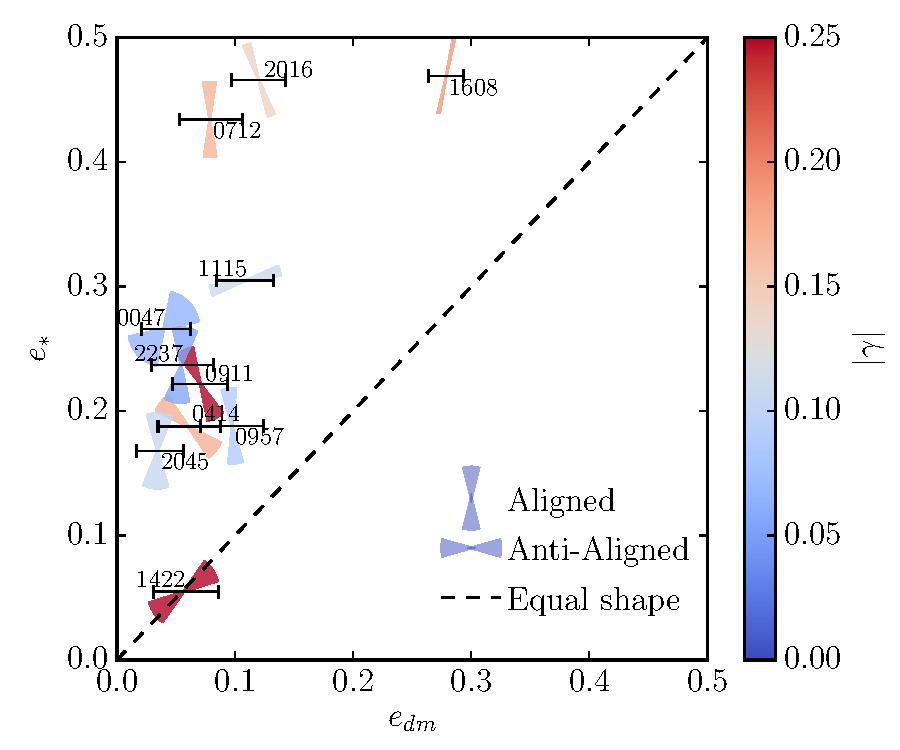
\includegraphics[width=.8\linewidth]{Figures/wedges_shears.pdf}
  \caption[width=\linewidth]{The reconstructed lenses are displayed according to the reconstructed total shapes of the dark matter halo $s_{dm}$ and the stellar component $s_{*}$. The wedges display the alignment of the semi-major axes of the components. In case of alignment of the semi-major axes (Aligned), the wedges are vertical. In case of alignment of the semi-major with the semi-minor axes (Anti-Aligned), the wedges are horizontal. The opening angle displays the statiscal error in the shape estimate of the dark matter halo. Both the error in the alignment and the ellipticity of the dark matter distribution denote the ranges $68\%$ of all the mass models lie within. The lenses are additionally color-coded in terms of the required external shear in modelling the lens.}
  \label{fig:wedgesall}
\end{figure*}

\begin{figure*}
  \centering
  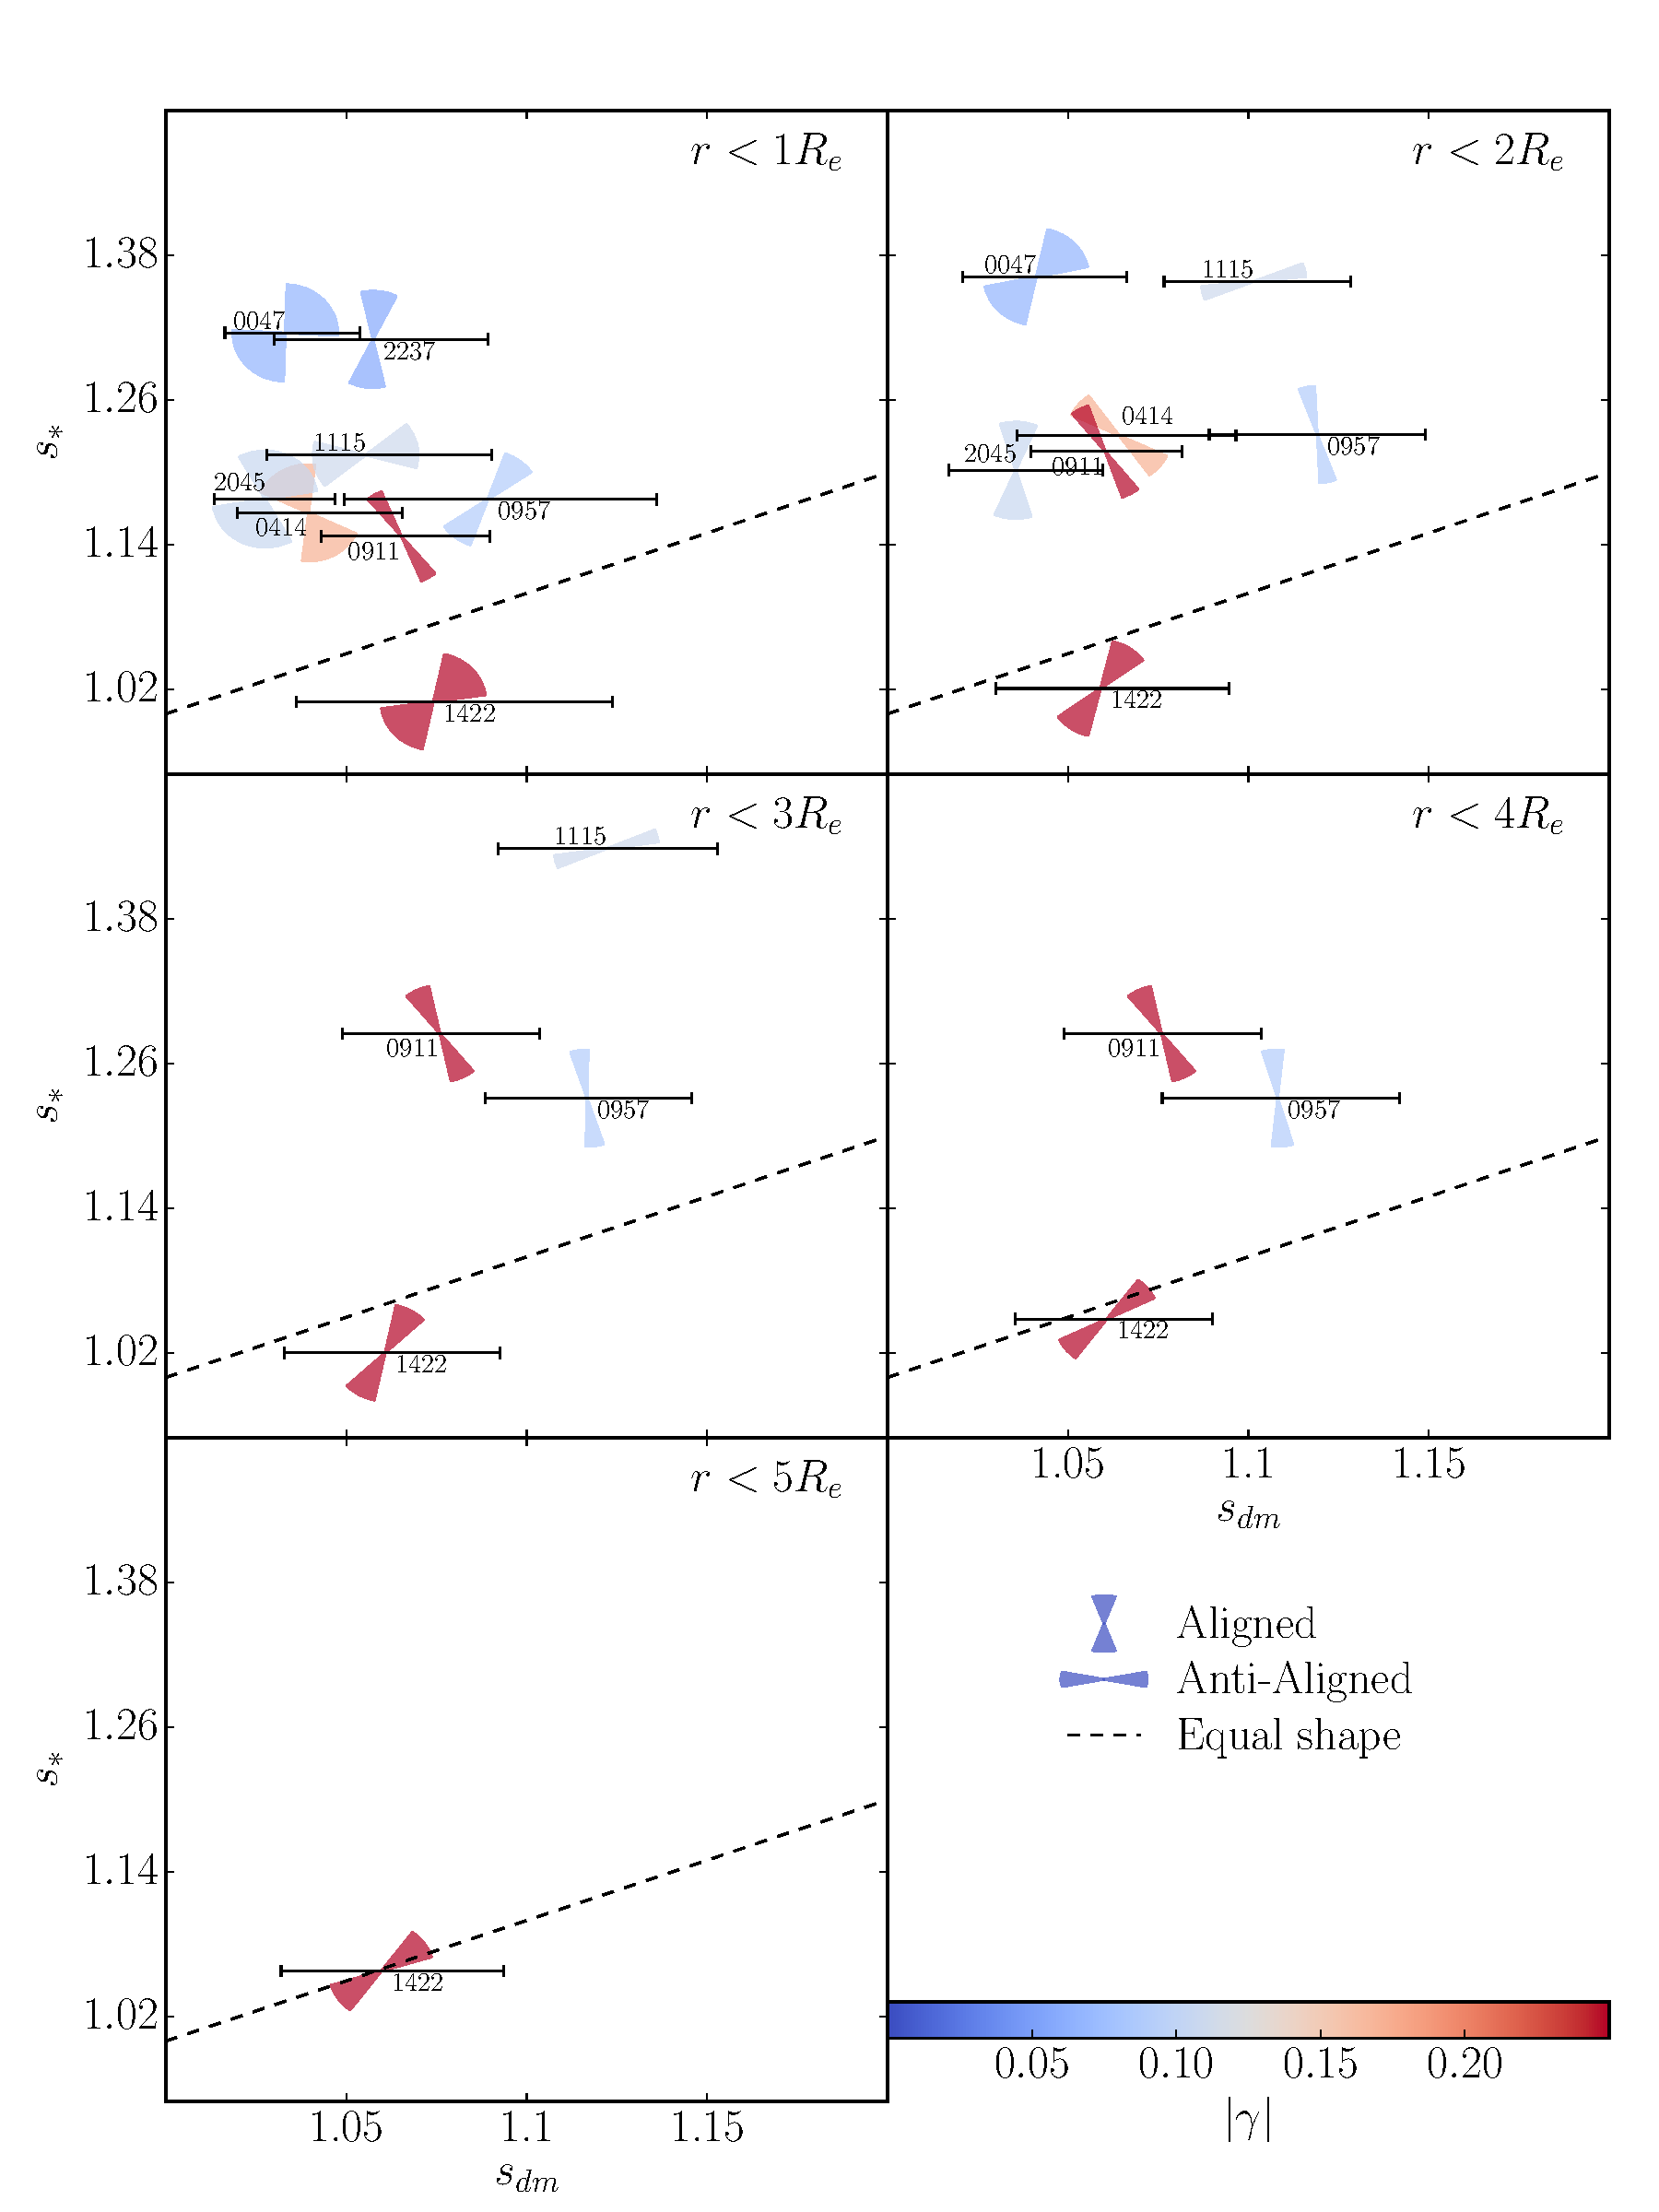
\includegraphics[width=.8\linewidth]{Figures/wedges.pdf}
  \caption[width=\linewidth]{Similar to Figure~\ref{fig:wedgesall}. In each of the subfigures however we only consider pixels within 1, 2, 3, 4, or 5 $R_e$. If the outermost image of a system lies within one of the limiting radii, the system is kept in this panel, but dropped from subsequent panels.}
  \label{fig:wedgesradii}
\end{figure*}

We have applied \Glass\ to the data set described in \S\ref{sec:data} consisting of 11 lenses. The reconstructed stellar and dark mass maps for each individual lens are given in the Appendix.

Figure~\ref{fig:wedgesall} shows our results for the shapes (see \S\ref{sec:shapemethod}) and alignments of the dark and stellar mass distributions. In this Figure, the full distribution up to the last-image radius $R_{L}$ is probed. There are several key points to note. Firstly, the reconstructed dark matter distribution of all lenses considered here is rounder than the stellar distribution. Secondly, most lenses lie in the bottom-left corner: the dark matter distributions are typically quite round, while the stellar distributions can be rather elliptical. Thirdly, 3 out of the 11 systems, {\it0712}, {\it2016}, and {\it1608}, stand out due to their larger stellar ellipticity ($s_* > 1.6$). At the same time, they show a very strong alignment between their dark matter and stellar distributions. One of these lenses ({\it1608}) is an known merger of an early-type galaxy with a probable late-type galaxy \citep{2003ApJ...584..100S}. We suggest that the other two systems, {\it0712} and {\it2016}, may also be post-merger systems, explaining their similarities with {\it1608}. Fourthly, notice that all dark matter and stellar distributions with weak shear (see the contour bar that displays the shear $\gamma$) are aligned apart from {\it0047} which is almost spherical ($s_{dm}\sim1.05$). By contrast, systems requiring a larger external shear ({\it0414}, {\it0911}, and {\it1422}) can display a sizeable misalignment between the distributions. The latter two systems are located in dense environments (see Table~\ref{tab:lensproperties}) that are likely responsible for these misalignments. Two systems stand out from the rest, however. In {\it1115}, the semi-major axis of the dark matter seems to be aligned with the semi-minor axis of the stellar component; it is the most strongly misaligned system of all lenses studied here. This may be explained by its external shear ($\gamma \sim 0.1$) that likely owes to its group environment (see Table \ref{tab:lensproperties}). The lens {\it0414} is also interesting. It also shows strong misalignment, yet has no sign of a group or cluster environment reported to date. It does show rather strong external shear, however ($\gamma \sim 0.15$), suggesting that a group or cluster environment perhaps remains to be found.

We performed tests for the robustness of our shape estimate and its dependence, in particular, on the shear prior. Only two systems, {\it1422} and {\it2045}, reacted to a stricter prior on the external shear $|\gamma|$. {\it1422} requires a rather large external shear ($|\gamma|\sim0.25$). Restricting the range of the allowed external shear values did not affect the misalignment of the dark matter and stellar mass distributions. It did, however, increase the ellipticity of the reconstructed mass distribution: we observed a trade-off between the galaxy's ellipticity and the magnitude of the external shear as might be expected. {\it2045} on the other hand is particularly interesting. Allowing the shear to roam free as for the other lenses, favours an anomalously high shear ($\gamma > 0.5$), with strong misalignment. However, such models also produce spurious extra images along the arc. We find that limiting the maximum shear $|\gamma|$ to 0.1 removes the extra images, though the lens then pushes on its maximum shear prior. We find that the mass map is robust against a stronger shear prior, and it thus again does not affect the alignment of the distributions. It produces dark matter distributions well-aligned with the stars. We believe that a strong shear prior for this particular lens is justified by the non-observation of the spurious extra images; none of the other lenses in our sample have a shape profile that is sensitive to our shear prior.

Figure~\ref{fig:wedgesradii} is similar to Figure~\ref{fig:wedgesall} with the difference that shapes are now averaged within different multiples of $R_e$. Most lenses show a $\sim$ constant shape with radius appearing similar to the results in Figure~\ref{fig:wedgesall}. {\it0957} and to some degree {\it1422} display, however, some signs of isophotal twist (see also Appendix). Additionally, there appears to be a trend that the ellipticity of the stars and potentially of the dark matter (though the latter is consistent with constant ellipticity) increases with increasing radius.

\section{Conclusions}\label{sec:conclusions}
We have measured the shape and alignment of stars and dark matter in 11 strong lensing galaxies using a new non-parametric lens tool, \Glass. We focussed on lenses that have either time delay data or stellar mass maps that contribute significantly to the central potential, since these have data quality good enough to determine the projected shape of their dark matter halos \citep{2014arXiv1401.7990C}. We measured the shape and alignment using the eigenvalues $\lambda$ and vectors of the 2D moment of inertia tensor of the stars and dark matter, defining a {\it shape parameter} $s = \lambda_{\rm max}/\lambda_{\rm min}$ (\S\ref{sec:shapemethod}). We averaged $s$ over the range 1-5$R_e$, where $R_e$ is the effective radius of the light profile.

Our key results are as follows:

\begin{itemize}
\item We found that in all cases the dark matter halos are rounder than the light distribution over the range $R_e < R < 5R_e$. As we average over larger radii, the lenses become increasingly elliptical in their stars and potentially dark matter, but dark matter halos are never more elliptical than $s_{dm} = 1.15$, while their stars can extend to $s_* > 1.4$. 

\item Three systems have very high stellar ellipticity ($s_* > 1.6$) and correspondingly high alignment between light and dark. One of these -- {\it1608} -- is a known merging pair; we suggest that the other two ({\it0712} and {\it2016}) may also be recent post-merger systems. 

\item Galaxies with high dark matter ellipticity and weak external shear show strong alignment between light and dark; those with strong shear ($\gamma \simgt 0.1$) can be highly misaligned. This is reassuring since isolated misaligned galaxies are expected to be unstable.
\end{itemize}

Our results provide a new constraint on galaxy formation models that must explain the origin of very round dark matter halos (not expected in pure dark matter only simulations), and highly misaligned systems. Such misalignments also present a new challenge for alternative gravity theories in which the light and dark must necessarily be highly correlated.

\section{Acknowledgements}\label{sec:acknowledgements}
JIR would like to acknowledge support from SNF grant PP00P2\_128540/1.

\bibliographystyle{mn2e}
\bibliography{paper}

\appendix
\section{Reconstructed Lenses}\label{sec:reconstructions}
\begin{table}
  \begin{center}
    \begin{tabular}{l r r r r}
      Lens & A [''] & B [''] & C [''] & D [''] \\ \hline
      0047 & 1.270 & -0.630 & 0.520 & -0.730 \\
           & 0.105 & -0.995 & -1.045 & 0.705 \\
      0414 & -0.472 & -1.061 & -1.1947 & 0.885 \\
           & 1.277 & -0.661 & -0.255 & -0.361 \\
      0712 & -0.013 & 0.795 & 0.747 & -0.391 \\
           & -0.804 & -0.156 & -0.292 & 0.307 \\
      0712 & -0.013 & 0.795 & 0.747 & -0.391 \\
           & -0.804 & -0.156 & -0.292 & 0.307 \\
      0957$^{a}$ & 1.408 & 0.182 & 2.860 & -1.540 \\
           & 5.034 & -1.018 & 3.470 & -0.050 \\
      1115 & 0.355 & -0.909 & -1.093 & 0.717 \\
           & 1.322 & -0.714 & -0.260 & -0.627 \\
      1422 & 1.079 & 0.357 & 0.742 & -0.205 \\
           & -0.095 & 0.973 & 0.656 & -0.147 \\
      1608 & -1.300 & -0.560 & -1.310 & 0.570 \\
           & -0.800 & 1.160 & 0.700 & -0.080 \\
      2016 & -1.735 & 0.335 & 0.437 & 1.268 \\
           & 1.778 & -1.450 & -1.435 & 0.276 \\
      2045 & 1.121 & 1.409 & 1.255 & -0.507 \\
           & 0.824 & 0.035 & 0.576 & -0.183 \\
      2237 & 0.598 & -0.075 & 0.791 & -0.710 \\
           & 0.758 & -0.939 & -0.411 & 0.271 \\
    \end{tabular}
    \caption[width=\linewidth]{The image positions of all the systems in order of arrival time (image A has the shortest arrival time, image D the longest) are listed. The positions are relative to the center of the lens galaxy. The first row contains the RA coordinate, the second the DEC coordinate of the image. \newline $^{a}$ The source lensed by 0957 has different component. Images A and B are a double associated with the main galaxy component, images C and D are associated with lensed substructure.}
    \label{tab:lenspositions}
  \end{center}
\end{table}

In this Appendix, we show the results of our lens modelling for each individual lens (Figures~\ref{fig:lensreconstruction1}-\ref{fig:lensreconstruction3}). The panels show, from left to right: the arrival time surface; the surface mass density of the dark matter; and the surface mass density of the stars. The solid lines mark the eigenvalues and eigenvectors of the 2D moment of inertia tensor in each case; the dotted lines the 68\% confidence interval of these for the dark matter map. Figure \ref{fig:wedgesall} is constructed from the ratio of largest to smallest eigenvalue in each case (to measure the shape parameter $s$), and the angle between the dark matter and stellar major axes. Note that the angular scale is always the same for the dark matter and stellar maps, but varies between the different lenses as marked on the Figure axes.

We note in Figure~\ref{fig:lensreconstruction2} specifically for {\it0957} and to some degree also {\it1422} twisting isophotes \citep{1978ComAp...8...27B}. {\bf (CB: DOES THIS NEED TO BE EXPANDED?)}

\begin{figure*}
  \centering
  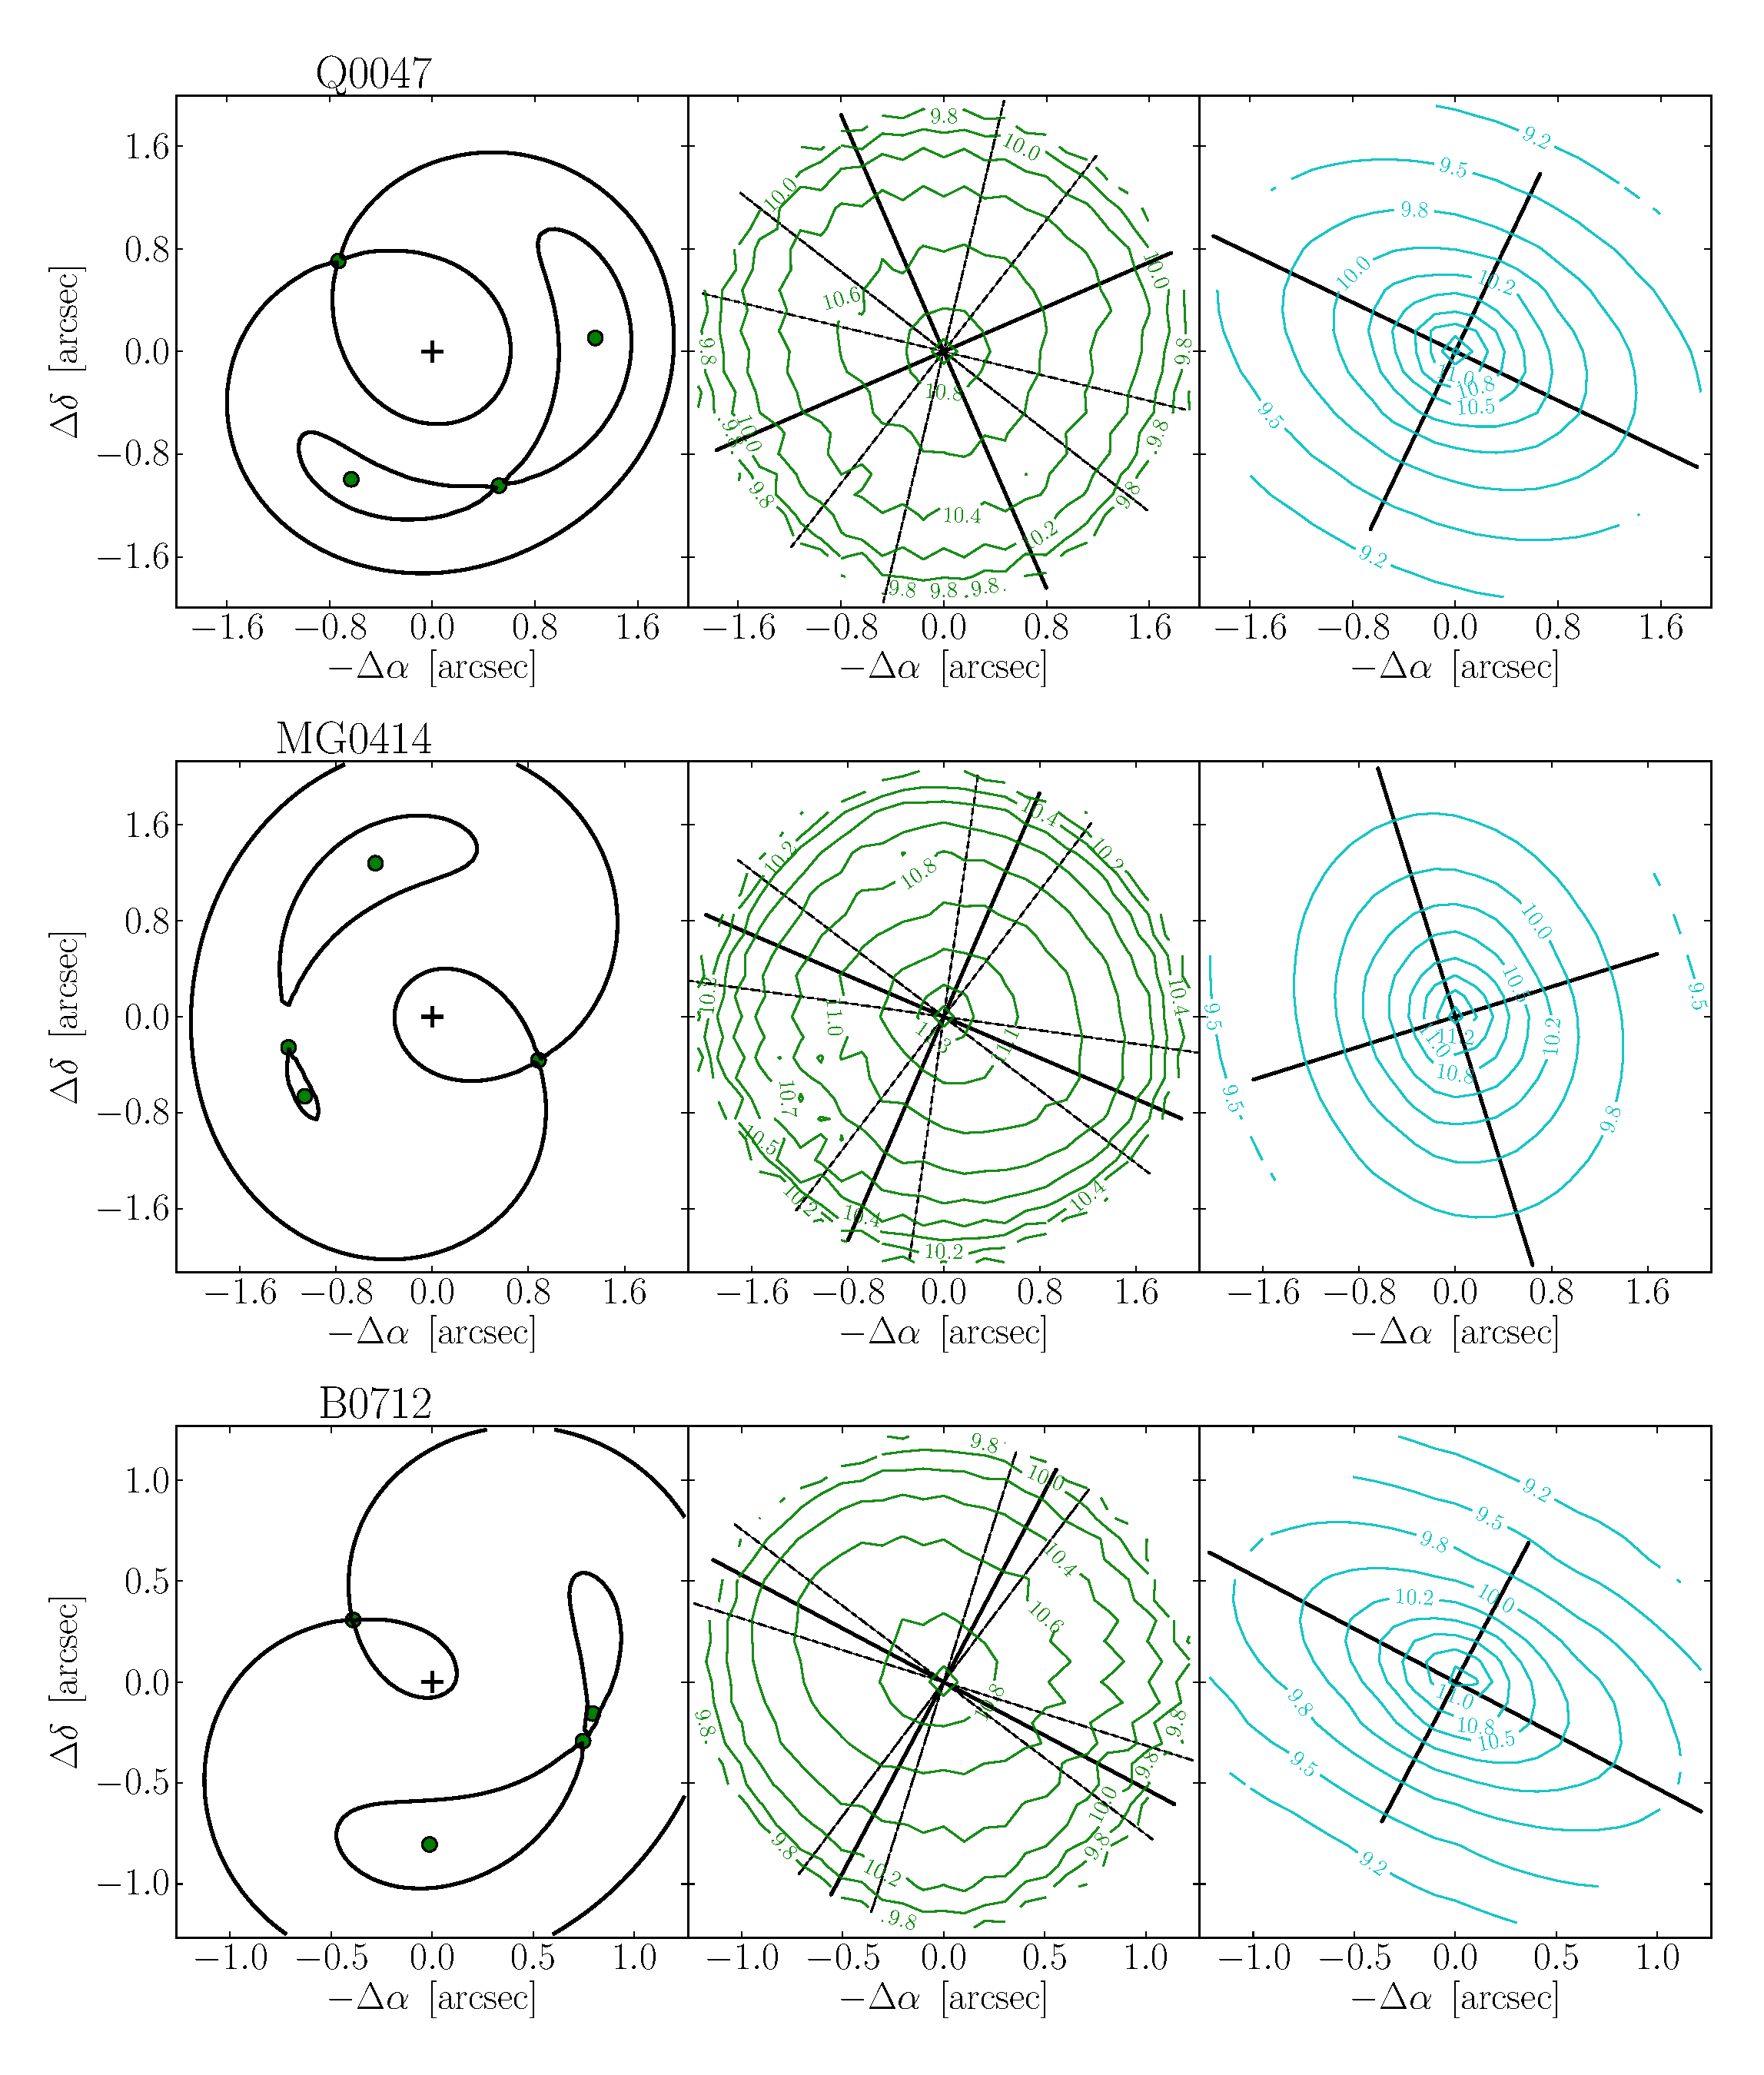
\includegraphics[width=.8\linewidth]{Figures/AllLenses31.pdf}
  \caption[width=.65\linewidth]{The results of our lens modelling for each individual lens. The panels show, from left to right: the arrival time surface (the images are marked by the green circles); the surface mass density of the dark matter; and the surface mass density of the stars. The solid lines mark the eigenvalues and eigenvectors of the 2D moment of inertia tensor in each case; the dotted lines the 68\% confidence interval of these for the dark matter map.}
  \label{fig:lensreconstruction1}
\end{figure*}

\begin{figure*}
  \centering
  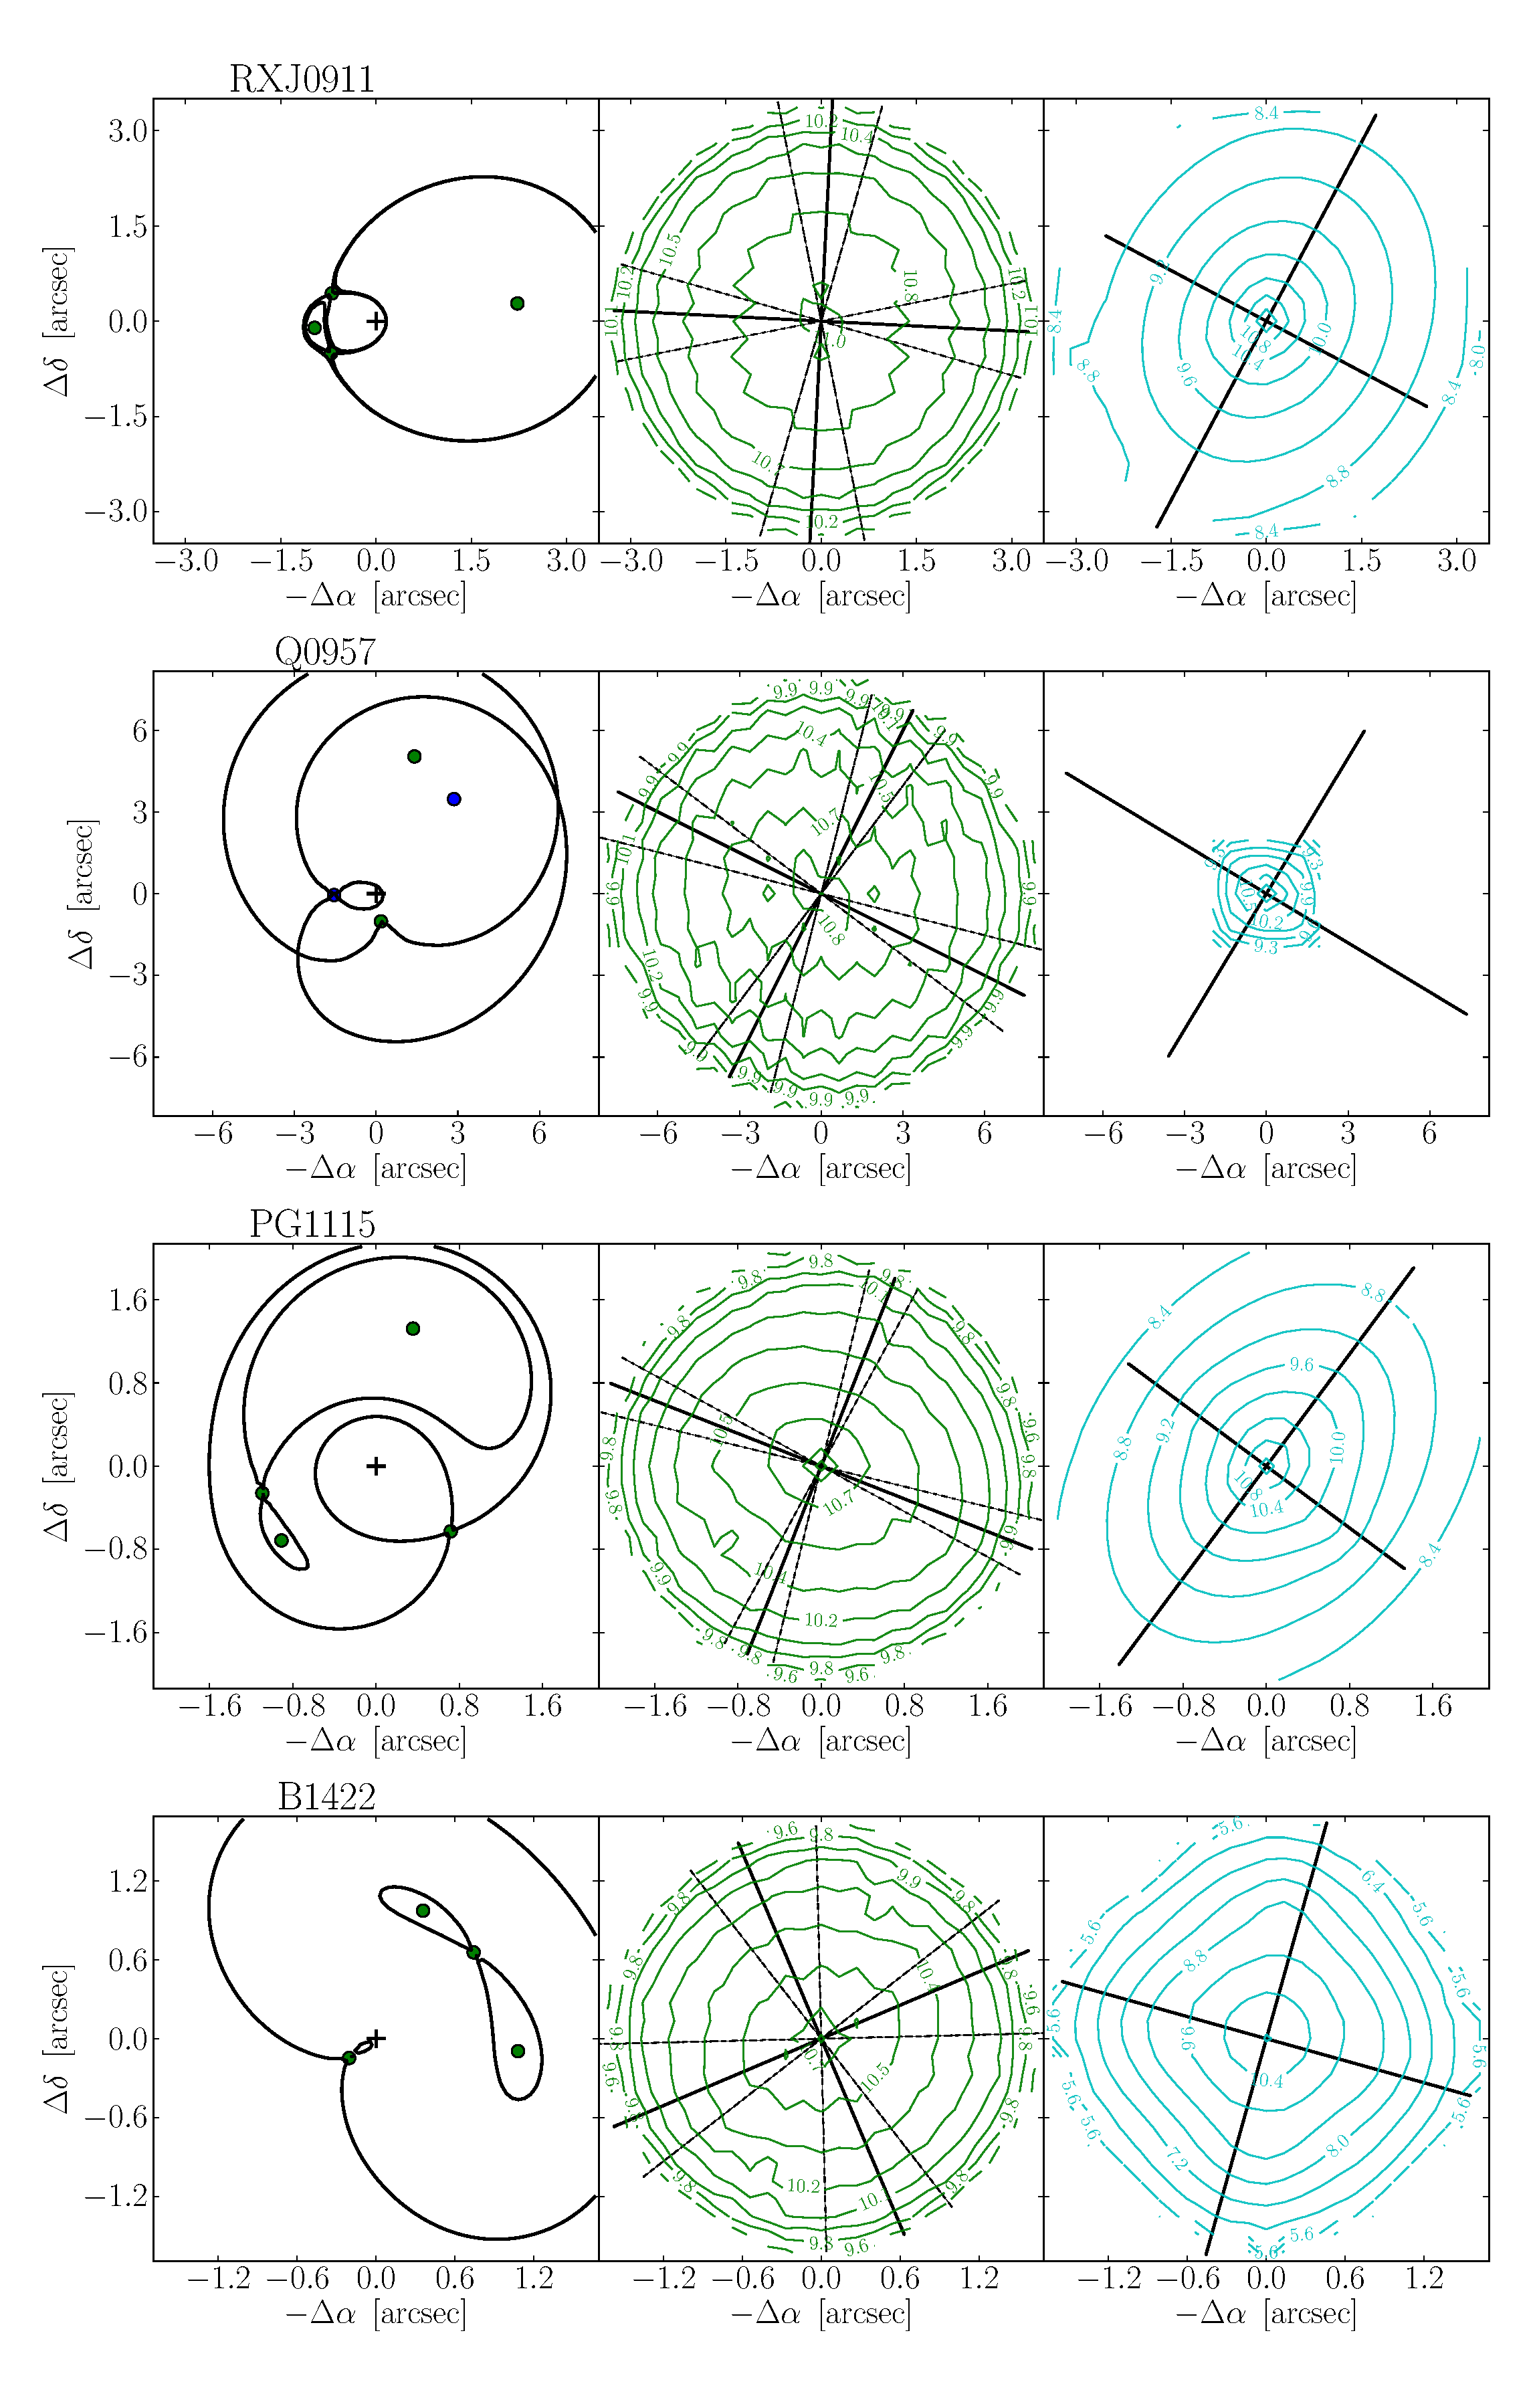
\includegraphics[width=.8\linewidth]{Figures/AllLenses32.pdf}
  \caption[width=.65\linewidth]{The results of our lens modelling for each individual lens. Lines and symbols are as in Figure \ref{fig:lensreconstruction1}.}
  \label{fig:lensreconstruction2}
\end{figure*}

\begin{figure*}
  \centering
  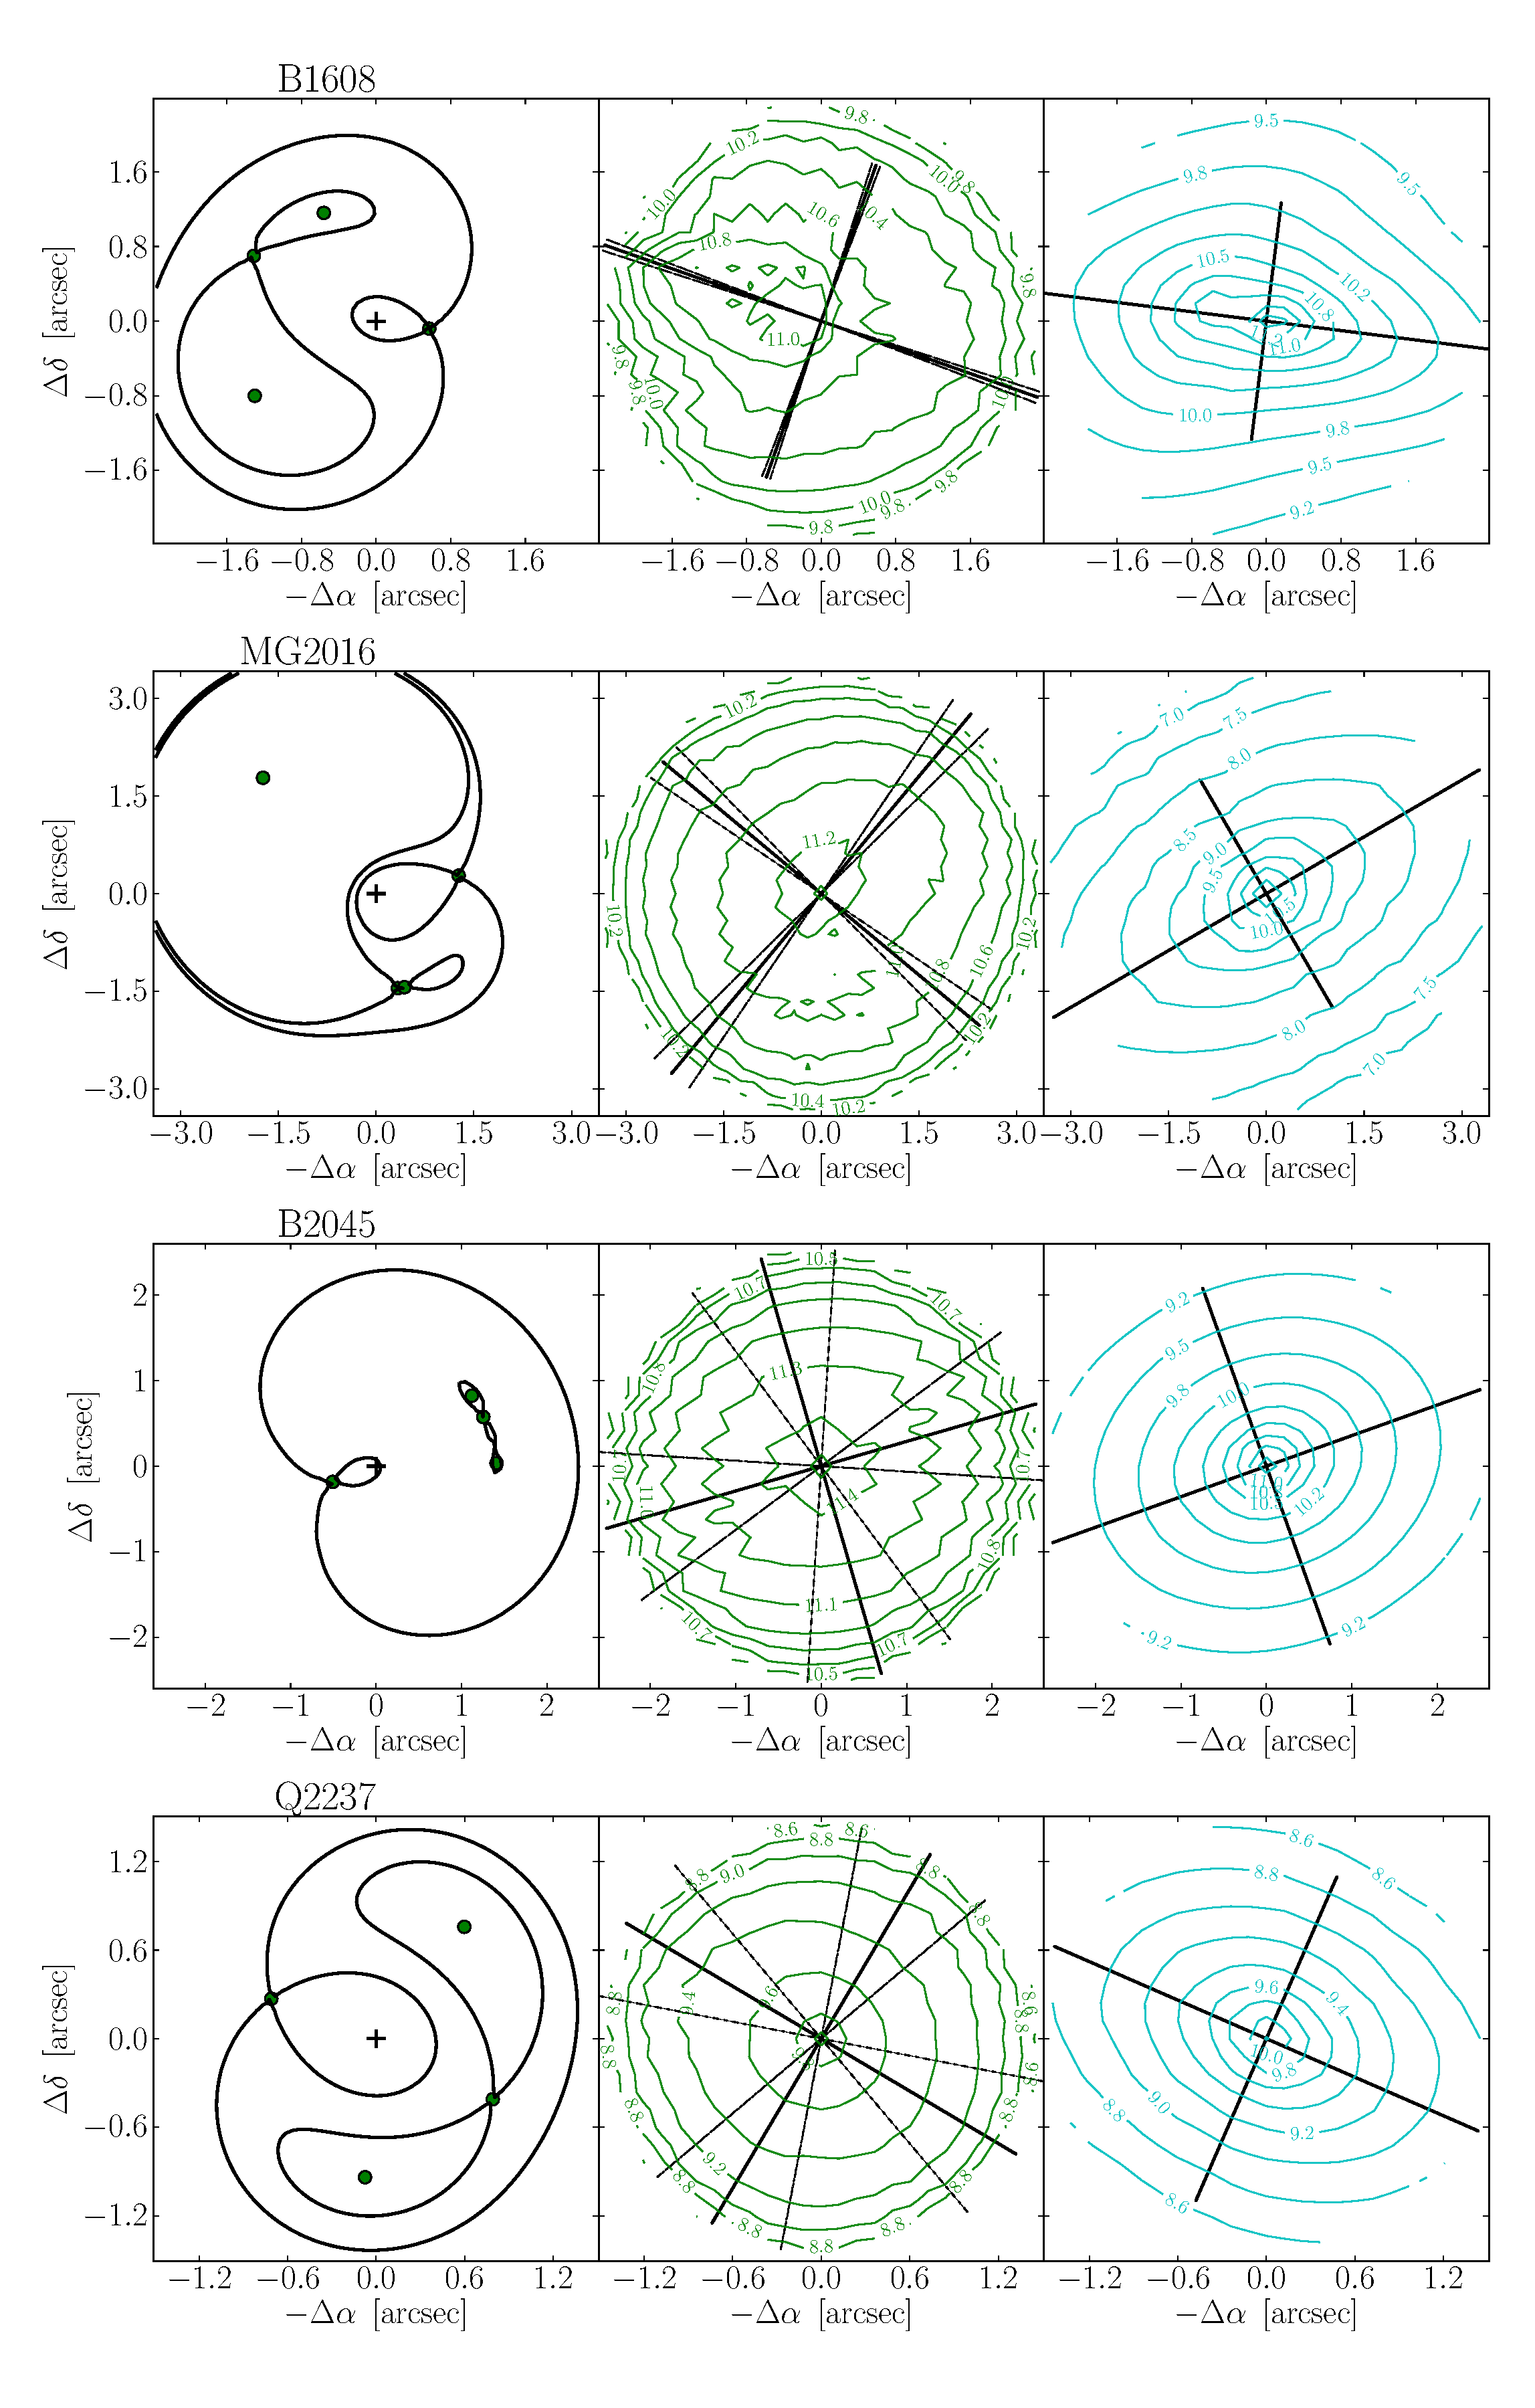
\includegraphics[width=.8\linewidth]{Figures/AllLenses33.pdf}
  \caption[width=.65\linewidth]{The results of our lens modelling for each individual lens. Lines and symbols are as in Figure \ref{fig:lensreconstruction1}.}
  \label{fig:lensreconstruction3}
\end{figure*}

\end{document}
